% Section content template for individual Educative lessons
% This file contains the actual content for a specific section
% Generated from Educative API section content

% Section: Getting Ready: Amazon Locker Service
% Section ID: 6069894208815104
% Section Slug: getting-ready-amazon-locker-service
% Generated: 2025-12-11T15:16:29.335220

\subsection{Problem definition}\label{8t8osGei0gD63dyNYRfeL-1}
\\
\textbf{Amazon} is an online retailer that allows customers to order products for delivery. Sometimes, customers are unavailable at their usual address to receive packages. In such cases, Amazon provides a secure, automated pickup and return service called \textbf{Amazon Locker}.
\\
Amazon Lockers are available at various locations, each containing multiple lockers of different sizes and operating hours. Customers can select a nearby locker location for delivery or returns. Only packages that fit a locker's size are eligible. When a package arrives, the customer receives a unique code to retrieve it. Packages are stored for a limited period; if uncollected, they are removed, and the customer may be refunded. Customers can also return eligible products by dropping them off at available locker locations, where the logistics team picks them up.
\\
This scenario presents interesting challenges: real-time resource allocation, handling concurrent user requests, operating hour constraints, managing physical locker and package sizes, and supporting delivery and return flows.
\\
In this LLD interview case study, you'll focus on:

\begin{itemize}
\item
\protect\phantomsection\label{2EJBSmqU2syYVl9AenZbC}
Assigning lockers to orders and returns based on size and availability.
\item
\protect\phantomsection\label{00hrexJ79xVCs2zGAYH3P}
Handling package pickups, returns, and uncollected items.
\item
\protect\phantomsection\label{_RAu-Gb169EKU3Fz2Kqzq}
Managing locker states, codes, and access windows.
\item
\protect\phantomsection\label{xrZ7qnoD9HgqU7cYagVHj}
Ensuring the system works reliably and securely at scale.
\end{itemize}
\\
This system model can be adapted for any retailer providing automated, secure delivery and returns.

\begin{figure}[htbp]
 \centering
 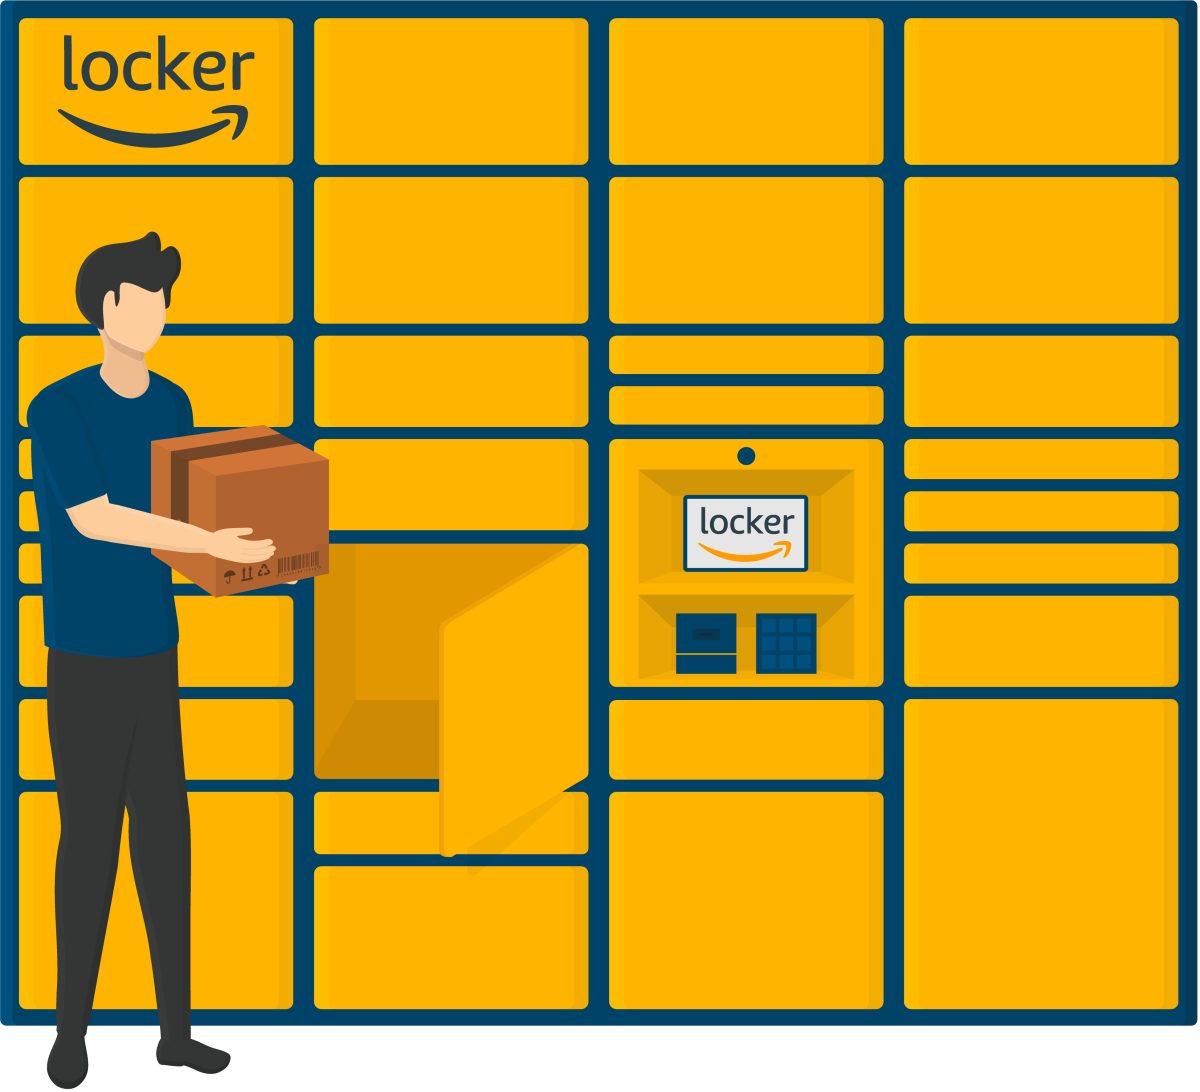
\includegraphics[width=0.25\textwidth]{Images/chapter_10/section_6069894208815104/6294617370918912.png}
 \caption{The Amazon Locker service}
\end{figure}

\subsection{Expectations from the interviewee}\label{8t8osGei0gD63dyNYRfeL-2}
\\
The Amazon Locker service consists of multiple components, each with functionality and constraints. The following section provides an overview of some of the main expectations the interviewer will want to hear you discuss in more detail during the interview.
\\
In the interview, you are expected to:

\begin{itemize}
\item
\protect\phantomsection\label{4s2w8VHbw7MriX499r8DJ}
Clarify system requirements, constraints, and edge cases by asking relevant questions.
\item
\protect\phantomsection\label{VlXzhQUqN7wYT48RSZa8Z}
Identify and design core system components.
\item
\protect\phantomsection\label{nyGvVdOTNO5gpAPJqN3O4}
Justify design decisions using OOD and SOLID principles.
\end{itemize}
\\
Typical areas you should probe and discuss include:

\subsubsection{Locker size}\label{CxCPbRSs21A2tuRHJusxQ}
\\
Every locker is of a specific size in the Amazon Locker system. The interviewer expects you to ask the questions listed below:

\begin{itemize}
\item
\protect\phantomsection\label{MQYRKOD3wtTwQkO3X_qlH}
Are there different locker sizes? How does package size affect locker assignment?
\item
\protect\phantomsection\label{vfkue2ppakhNdVhaYWLZn}
Are there restrictions on what can be stored in each locker?
\end{itemize}

\subsubsection{Locker selection}\label{CIqvzGObCrqWqqJxGH0sd}
\\
The most significant part of the Amazon Locker service is the selection of the locker. The system has to ensure that more than one customer cannot access a locker at the same time. The interviewer expects you to ask the questions listed below to identify how the system will work in such situations:

\begin{itemize}
\item
\protect\phantomsection\label{Xgnx0qktFm9M9kW4vwSEP}
How will the system ensure multiple customers do not get the same locker?
\item
\protect\phantomsection\label{0NoKBCFwxR00SJAr9MT5X}
Will the customer choose the locker of his own choice, or will the system assign him a locker based on availability?
\item
\protect\phantomsection\label{q2KrwWQLPTshJW-ct99tA}
Can a customer get two lockers for different orders at the same time?
\item
\protect\phantomsection\label{DjD0HpvDQkl6LZbLm-RVs}
Will the system consider the locker and package sizes while assigning the locker to the customer?
\end{itemize}

\subsubsection{Locker status}\label{IUVLxJ2I6kqFVOzbd8z5b}
\\
As this problem revolves around the locker, you may ask the questions listed below about the locker status:

\begin{itemize}
\item
\protect\phantomsection\label{fYSxOPi94kUDAv4d_JX3H}
Is there any time constraint on the package that can be kept in the locker?
\item
\protect\phantomsection\label{G9kuY3XeGv-58Z03Jgn0E}
What will happen if the customer does not come to pick up his package within the valid time period?
\end{itemize}

\subsubsection{Returning an item}\label{VtANmyUgKnpIYMCLsPfl_}
\\
Like the order delivery process, the item can be returned through the Amazon Locker service. Therefore, you may ask the questions listed below:

\begin{itemize}
\item
\protect\phantomsection\label{6kZPLOJlSsRQeNEcaNqYb}
Can the customer return an item through the Amazon Locker service?
\item
\protect\phantomsection\label{IT015xIOv3sTyuVwGnFgX}
If yes, will they get the same locker from which they picked the item?
\item
\protect\phantomsection\label{uaNecPaf6gWeATRM6shap}
How will the locker be assigned to the customer while returning an item?
\end{itemize}

\subsection{Design approach}\label{GBiPcFE-kg589jli7jhKf}
\\
We will design this Amazon Locker service using the bottom-up design approach. For this purpose, we will follow the steps below:

\begin{itemize}
\item
\protect\phantomsection\label{om5UK9I0GvZvIU3ZD-S7L}
First, we'll identify core entities like \texttt{Locker}, \texttt{LockerLocation}, \texttt{Package}, and \texttt{Order}, and define their responsibilities.
\item
\protect\phantomsection\label{vcLUWqL_4jnuwQgvRxdb9}
Next, we'll model how lockers are assigned to packages based on size and availability, and handle package pickups, returns, and uncollected items.
\item
\protect\phantomsection\label{XWYNnxjak2cyO3XwDLaSN}
We'll ensure that locker operations respect time limits and location operating hours and support secure access via unique codes.
\end{itemize}
\\
This design approach will address concurrency and edge cases and follow SOLID principles to ensure scalability and maintainability. Later , diagrams and code will illustrate major workflows and class structures.

\subsection{Design pattern~}\label{sMziTama7-nHQurh5LN7C}
\\
During an interview, discussing the design patterns under which the Amazon Locker system falls under is always a good practice. Stating the design patterns gives the interviewer a positive impression and shows that the interviewee is well-versed in the advanced concepts of object-oriented design.
\\
Try to answer the following question. If you are not familiar with design patterns, don't worry! You can learn about them by asking ``Define design patterns.''

\textbf{Question:}

Which design pattern(s) should be used to design an Amazon Locker service? Kindly elaborate on your choice(s).

Let's explore the requirements of the Amazon Locker service in the next lesson.

% End of section content